\documentclass[12pt,a4paper]{article}
\usepackage[spanish]{babel}
\usepackage[margin=2.5cm]{geometry}
\usepackage{graphicx}
\usepackage{fancyhdr}
\usepackage{hyperref}
\usepackage{float}
\usepackage{amsmath}
\usepackage{xcolor}
\usepackage{setspace}

% Configuración de espaciado
\onehalfspacing

% Encabezado y pie de página
\pagestyle{fancy}
\fancyhf{}
\rhead{\thepage}
\lhead{Informe de Realidad Aumentada}

% Colores personalizados
\definecolor{darkblue}{RGB}{0,51,102}
\definecolor{lightgray}{RGB}{240,240,240}

% Configuración de hiperenlaces
\hypersetup{colorlinks=true, linkcolor=darkblue, urlcolor=darkblue}

\title{}
\author{}
\date{}

\begin{document}

% ======================== PORTADA ========================
\begin{titlepage}
    \centering
    
    % Logo ESPE
    \vspace*{1cm}
    
\includegraphics[width=3cm]{images/Logo_ESPE.png}
    
    \vspace{1.5cm}
    {\Large \textbf{ESCUELA POLITÉCNICA NACIONAL}}
    
    \vspace{0.5cm}
    {\large Carrera de Ingeniería de Software}
    
    \vspace{3cm}
    
    % Título del proyecto
    {\LARGE \textbf{INFORME DE PROYECTO}}
    
    \vspace{0.5cm}
    {\Large \textbf{Modelo 3D de Mascota de Carrera con}}
    
    {\Large \textbf{Realidad Aumentada}}
    
    \vspace{3cm}
    
    % Información del estudiante y curso
    {\large
    \textbf{Estudiante:} Bryan Quispe \\
    \vspace{0.5cm}
    \textbf{Materia:} Desarrollo de Software Aplicado para el Dominio de Interculturalidad \\
    \vspace{0.5cm}
    \textbf{NRC:} 30745 \\
    \vspace{0.5cm}
    \textbf{Tutor:} Ingeniero Cristian Andrés Cola Pérez \\
    }
    
    \vfill
    
    % Fecha
    {\large Quito, Ecuador \\ \today}
    
\end{titlepage}

% ======================== TABLA DE CONTENIDOS ========================
\newpage
\tableofcontents
\newpage

% ======================== INTRODUCCIÓN ========================
\section{Introducción}

El presente informe documenta el desarrollo de un modelo tridimensional que representa la mascota oficial de la carrera de Ingeniería de Software, aplicando tecnología de realidad aumentada. Este proyecto combina habilidades de modelado 3D con herramientas modernas de visualización, permitiendo a los usuarios interactuar con el modelo mediante dispositivos móviles a través de códigos QR.

La realidad aumentada (AR) ha revolucionado la forma en que presentamos contenidos visuales. Este proyecto demuestra cómo la integración de esta tecnología con modelos 3D personalizados puede mejorar la experiencia del usuario y crear una conexión única con la identidad institucional.

% ======================== INSPIRACIÓN Y CONCEPTO ========================
\section{Inspiración y Concepto del Proyecto}

\subsection{Fuente de Inspiración}

La inspiración para este proyecto proviene del contexto humorístico y cultural de la comunidad de Sistemas. Se tomó como referencia una representación irónica y satírica que es ampliamente reconocida en círculos de profesionales de tecnología e informática.

\begin{figure}[H]
    \centering
    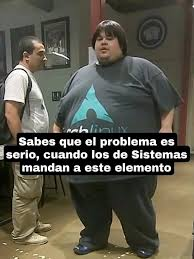
\includegraphics[width=0.6\textwidth]{images/imagen_referencia.png}
    \caption{Referencia de inspiración: Meme cultural de la comunidad de Sistemas}
    \label{fig:referencia}
\end{figure}

\subsection{Descripción del Modelo}

El modelo desarrollado representa un personaje masculino con características distintivas: una complexión particular y vestuario temático (camiseta con distribución de Archlinux), elementos que lo hacen reconocible y atractivo para la comunidad de desarrollo de software. La idea fue crear una mascota memorable que fusionara el aspecto humorístico con la identidad institucional.

% ======================== PROCESO DE MODELADO ========================
\section{Proceso de Modelado 3D}

\subsection{Descripción General}

El proceso de modelado se realizó completamente en un software de modelado 3D profesional, utilizando técnicas de modelado mesh y refinamiento de geometría. El proyecto fue completado en aproximadamente 4 horas de trabajo dedicado, incluyendo todas las fases de desarrollo.

\subsection{Desafíos Principales del Modelado}

Durante el proceso de creación, se presentaron desafíos técnicos significativos que requirieron atención especial:

\subsubsection{Modelado del Calzado}

Uno de los componentes más complejos fue la creación del calzado. El detalle de la geometría, la estructura tridimensional, el acabado y la proporción fueron aspectos críticos que demandaron precisión y múltiples iteraciones.

\begin{figure}[H]
    \centering
    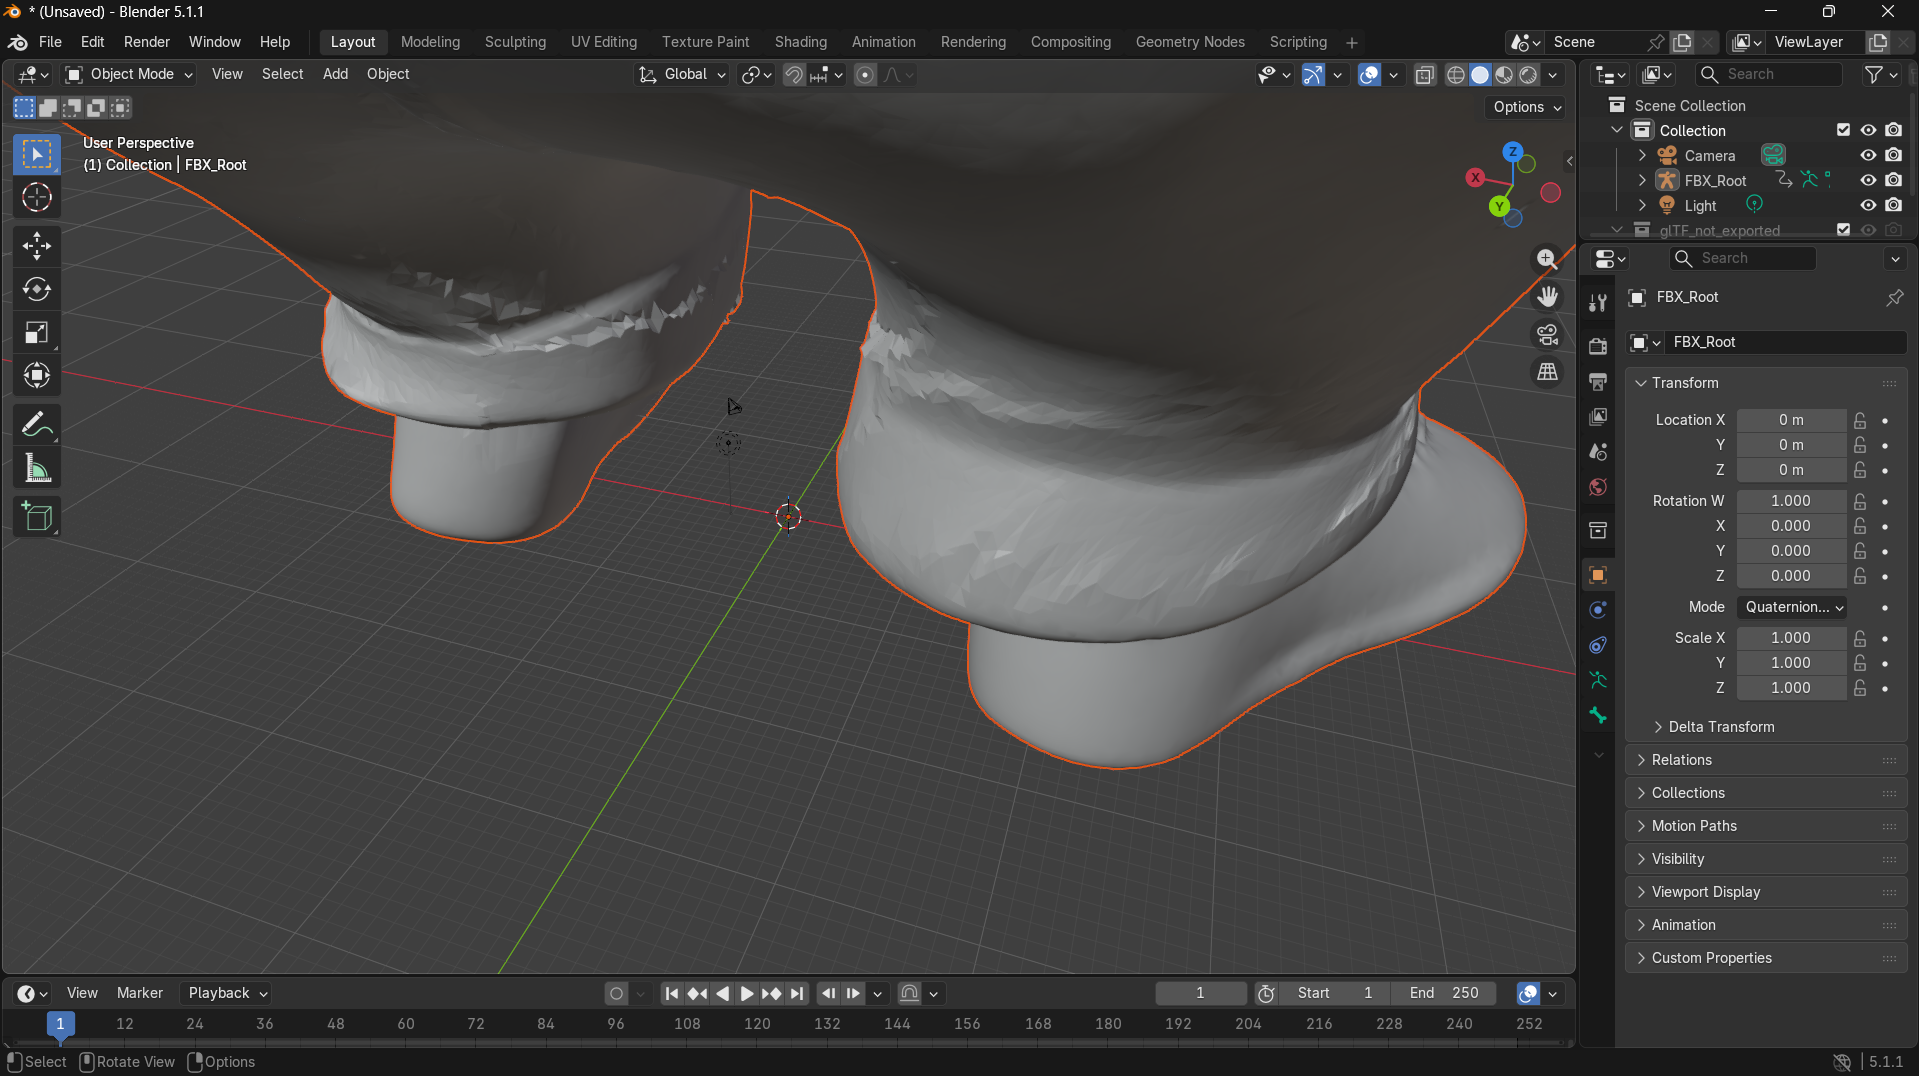
\includegraphics[width=0.5\textwidth]{images/modelado de zapatos.png}
    \caption{Detalle del modelado del calzado}
    \label{fig:zapatos}
\end{figure}

\subsubsection{Modelado de la Mochila}

La mochila presentó complejidades similares, requiriendo especial atención en la geometría de los compartimentos, correas y proporciones espaciales para lograr un resultado realista y coherente con el modelo general.

\begin{figure}[H]
    \centering
    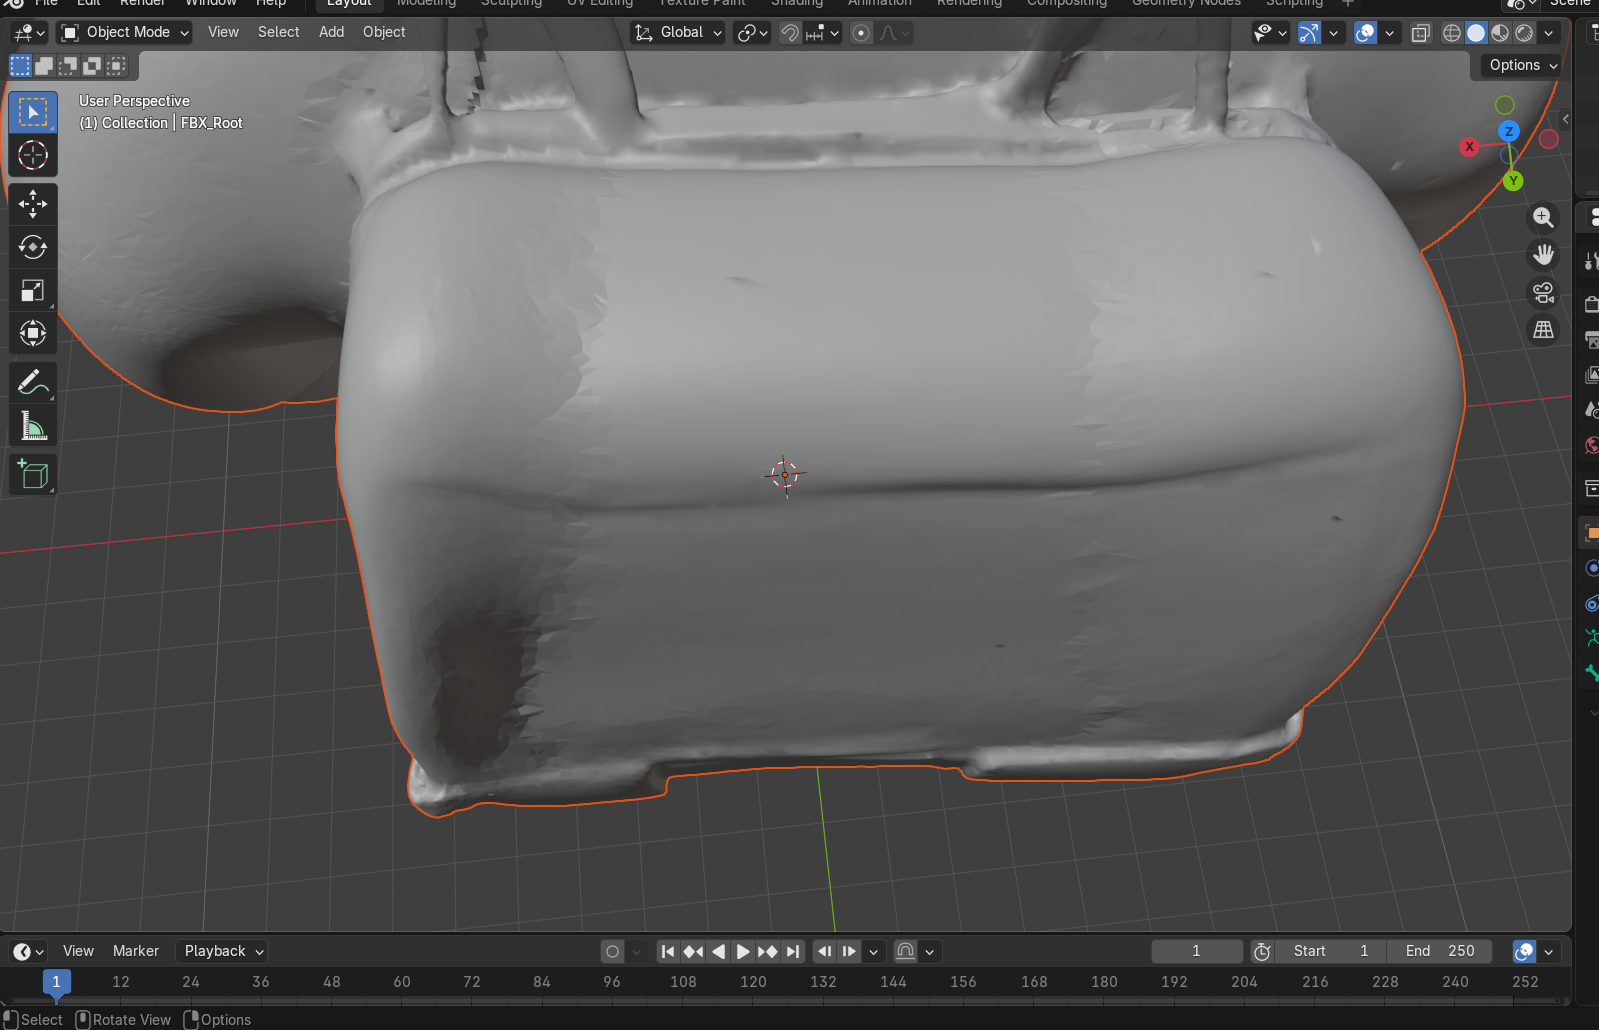
\includegraphics[width=0.5\textwidth]{images/modelado de mochila.png}
    \caption{Detalle del modelado de la mochila}
    \label{fig:mochila}
\end{figure}

\subsection{Resolución de Desafíos}

A pesar de las complejidades mencionadas, se logró obtener una figura con proporciones deseables y detalles satisfactorios dentro del tiempo establecido. El equilibrio entre calidad visual y eficiencia temporal fue fundamental para el éxito del proyecto.

% ======================== RESULTADO FINAL - MODELADO ========================
\section{Resultado del Modelado: Estructura Base}

Una vez completada la fase de modelado geométrico, se obtuvo una estructura tridimensional completa que cumple con los estándares de calidad esperados. A continuación se presenta el modelo en su forma base, sin aplicación de texturas.

\begin{figure}[H]
    \centering
    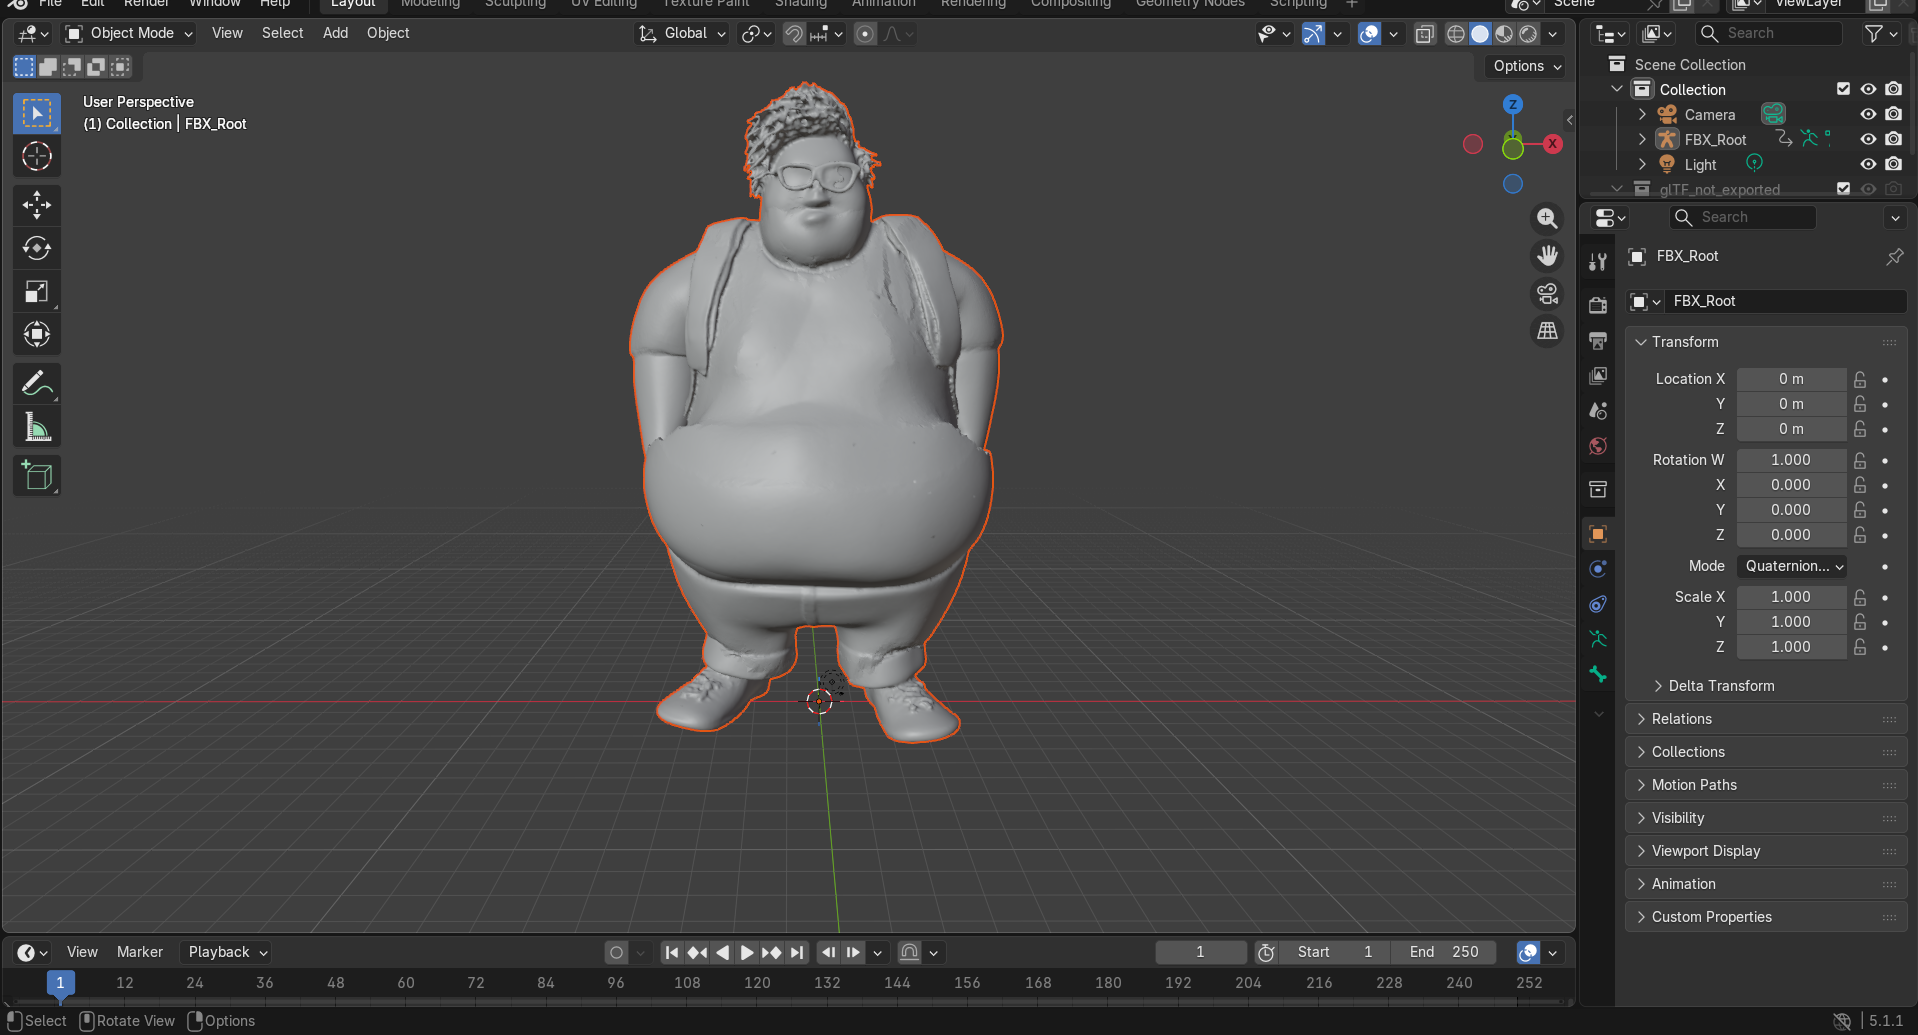
\includegraphics[width=0.7\textwidth]{images/MODELO_FINAL SIN TEXTURA.png}
    \caption{Modelo 3D final - Estructura base sin textura}
    \label{fig:modelo_base}
\end{figure}

Este estadio del proyecto representa la culminación del proceso de modelado, mostrando la precisión geométrica y la coherencia estructural del personaje.

% ======================== TEXTURIZACIÓN ========================
\section{Texturización y Visualización Final}

Una vez finalizada la estructura base del modelo, se procedió con la aplicación de texturas, materiales y colores para darle vida visual al proyecto. Este proceso incluye la asignación de propiedades de color, acabados superficiales y detalles visual adicionales.

\begin{figure}[H]
    \centering
    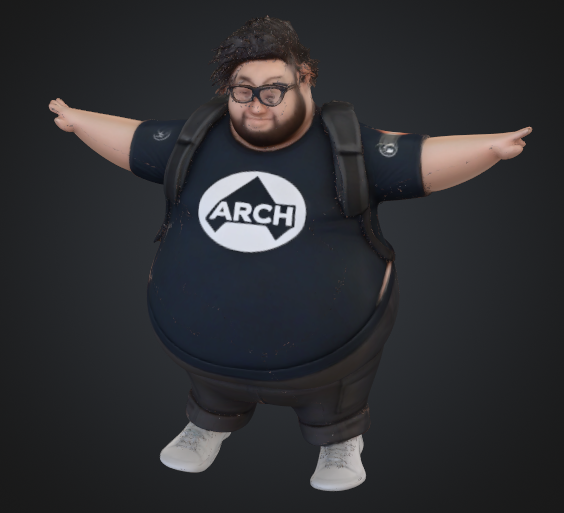
\includegraphics[width=0.7\textwidth]{images/Coloryrextura.png}
    \caption{Modelo 3D con textura y color aplicados}
    \label{fig:modelo_textura}
\end{figure}

La texturización fue esencial para mejorar el impacto visual del modelo, permitiendo una representación más cercana a la visión conceptual original y aumentando la atracción visual del proyecto final.

% ======================== REALIDAD AUMENTADA ========================
\section{Implementación de Realidad Aumentada}

\subsection{Integración de Tecnología AR}

El proyecto culmina con la integración de tecnología de realidad aumentada, permitiendo a los usuarios visualizar el modelo 3D en su entorno real a través de dispositivos móviles. La experiencia se activa mediante la lectura de un código QR especial.

\subsection{Código QR Interactivo}

Se ha generado un código QR animado que funciona como puerta de entrada a la experiencia de realidad aumentada. Al escanear este código con un dispositivo móvil compatible, los usuarios pueden visualizar el modelo tridimensional con movimiento y animaciones en tiempo real.

\begin{figure}[H]
    \centering
    \includegraphics[width=0.5\textwidth]{images/qr animado.jpeg}
    \caption{Código QR animado para acceder a la experiencia de Realidad Aumentada}
    \label{fig:qr}
\end{figure}

\subsection{Experiencia del Usuario}

Al escanear el código QR con un dispositivo móvil, el usuario accede a una experiencia interactiva donde:

\begin{itemize}
    \item El modelo 3D aparece superpuesto en su entorno real
    \item Se reproducen animaciones predefinidas del personaje
    \item Pueden interactuar con el modelo (rotación, zoom, etc.)
    \item La experiencia es totalmente intuitiva y accesible a cualquier usuario
\end{itemize}

% ======================== RESULTADOS Y LOGROS ========================
\section{Resultados y Logros}

\subsection{Objetivos Alcanzados}

\begin{itemize}
    \item Modelado completo de una mascota institutcional 3D con características distintivas
    \item Identificación y resolución de desafíos técnicos complejos (calzado y complementos)
    \item Aplicación profesional de texturas y materiales
    \item Integración exitosa de tecnología de realidad aumentada
    \item Generación de código QR funcional para acceso a la experiencia AR
    \item Optimización temporal (4 horas de trabajo efectivo)
\end{itemize}

\subsection{Impacto del Proyecto}

Este proyecto demuestra:

\begin{itemize}
    \item La viabilidad de crear experiencias inmersivas con herramientas modernas
    \item La importancia de la representación visual en la identidad institucional
    \item La capacidad de combinar modelado 3D con tecnología de realidad aumentada de manera efectiva
    \item La potencial aplicación de estas técnicas en otros contextos educativos e institucionales
\end{itemize}

% ======================== CONCLUSIONES ========================
\section{Conclusiones}

El desarrollo de este modelo 3D de la mascota de la carrera de Ingeniería de Software con integración de realidad aumentada representa un proyecto exitoso que combina creatividad, precisión técnica y aplicación de tecnología moderna.

A pesar de los desafíos presentados durante el modelado de elementos complejos como el calzado y la mochila, se logró completar un modelo de calidad satisfactoria en un tiempo razonable (4 horas). La posterior texturización y la integración de realidad aumentada elevaron el proyecto a un nivel de presentación profesional.

Este informe y el modelo asociado pueden servir como experiencia de referencia para futuros proyectos de visualización 3D e implementación de realidad aumentada dentro de la institución y la carrera.

% ======================== REFERENCIAS ========================
\section{Referencias}

\begin{enumerate}
    \item Tutoriales de Realidad Aumentada - \href{https://www.youtube.com/watch?v=O-tV7uBf5LI&t=830s}{https://www.youtube.com/watch?v=O-tV7uBf5LI}
    
    \item Modelado 3D con Blender - \href{https://www.youtube.com/watch?v=LcApcwU06mM}{https://www.youtube.com/watch?v=LcApcwU06mM}
    
    \item Playlist de Desarrollo de Software - \href{https://www.youtube.com/watch?v=GL2n20fkIeM&list=PLuSRwfbdkuG_bkepzBkCxYFopungXtsPJ}{https://www.youtube.com/watch?v=GL2n20fkIeM}
    
    \item Integración de Realidad Aumentada - \href{https://www.youtube.com/watch?v=bB8lpG7ZqRw}{https://www.youtube.com/watch?v=bB8lpG7ZqRw}
\end{enumerate}

\end{document}
